\documentclass[journal]{IEEEtran}

\usepackage{cite}
\usepackage{amsmath,amssymb,amsfonts}
\usepackage{algorithmic}
\usepackage{graphicx}
\usepackage{textcomp}
\usepackage{xcolor}
\usepackage{booktabs}
\usepackage{multirow}
\usepackage{url}
\usepackage{microtype}
\usepackage{bm}

\begin{document}

\title{DecisionSphere: A Calibrated Cross-Domain State-Space Architecture for Scenario-Based Strategic Planning and Risk Evaluation}

\author{P~Naga~Venkata~Kushal,
        P~Manjunatha~Kumar~Tejas,
        Jeswanth~Reddy~Sagabala,
        and~Dr.~Suresh~A%
\thanks{The authors are with the School of Computer Science and Engineering (SCOPE), Vellore Institute of Technology (VIT), Vellore, Tamil Nadu 632014, India (e-mail: kushal.pnv2023@vitstudent.ac.in; tejas.pmk2023@vitstudent.ac.in; jeswanth.rs2023@vitstudent.ac.in; suresh.a@vit.ac.in).}%
\thanks{This research was conducted under the B.Tech Computer Science and Engineering Capstone Project Program (BCSE497J -- Project I) under the faculty guidance of Dr. Suresh A.}%
}

\markboth{IEEE Transactions on Engineering Management,~Vol.~XX, No.~X,~October~2026}%
{Kushal \MakeLowercase{\textit{et al.}}: DecisionSphere: A Calibrated Cross-Domain State-Space Architecture}

\maketitle

\begin{abstract}
Strategic business decisions inherently trigger non-linear, cascading cross-domain consequences across modern enterprise operations. However, operational analytics systems exist almost universally within isolated functional silos: demand forecasting is confined to commercial sales teams, logistics delivery risk is isolated within fulfillment centers, and employee turnover is restricted to human resource departments. Consequently, commercial initiatives---such as promotional campaigns or rapid volume expansion---frequently induce unbuffered downstream operational friction, precipitating carrier delay fines, workforce overtime burnout, and catastrophic net operating margin collapse. In this paper, we introduce \textbf{DecisionSphere}, a computer-implemented decision intelligence platform that formalizes cross-domain enterprise coupling through a continuous 24-dimensional state-space vector $S_t \in \mathbb{R}^{24}$ and a topologically ordered Directed Acyclic Graph (DAG) state propagation operator. The architecture integrates three independently trained statistical machine learning estimators: an autoregressive XGBoost regressor for retail sales forecasting (Rossmann Store Sales benchmark), a post-hoc Platt-calibrated gradient boosted classifier for logistics delivery delay risk (DataCo Supply Chain benchmark), and a Platt-calibrated classifier for employee attrition risk under overtime strain (IBM HR Analytics benchmark). We establish a strict six-tier epistemic hierarchy that explicitly demarcates empirical ground truth, statistical model inferences, user scenario levers, propagated operational friction, deterministic accounting calculations, and lexicographic strategic recommendations, preventing causal hallucination and computational divergence. We evaluate the platform across ten formal research experiments (EXP-001 through EXP-010). Our empirical results prove that post-hoc Platt sigmoid scaling reduces Expected Calibration Error (ECE) from 0.0521 to 0.0142 (a 72.74\% error reduction), directly eliminating \$27,052.48 in contractual penalty calculation distortion. On an authoritative canonical commercial scenario (+15.0\% demand growth, active promotion, and 40.0\% mandatory overtime), DecisionSphere demonstrates that a projected commercial sales increase of +28,551.4 units generates +\$26,710.78 in incremental realized revenue yet induces +\$469,188.49 in logistics carrier fines and +\$184,212.00 in labor disruption expenses, collapsing net operating profit by -\$642,716.18 and inverting the strategic decision from an unbuffered commercial approval to an automated restructuring rejection (REJECT\_RESTRUCTURE, Composite Risk Score 37.48). Stochastic perturbation analysis across $N=50$ Monte Carlo runs demonstrates 100.0\% decision invariance under Gaussian noise, while computational sweeps verify strict $\mathcal{O}(N)$ linear runtime complexity with steady-state execution latencies of 275~ms to 945~ms per scenario.
\end{abstract}

\begin{IEEEkeywords}
Decision Intelligence, Cross-Domain Scenario Simulation, State-Space Modeling, Probability Calibration, Expected Calibration Error, Supply Chain Risk, Workforce Analytics, Directed Acyclic Graph, Explainable AI.
\end{IEEEkeywords}

\IEEEpeerreviewmaketitle

\section{Introduction}

\IEEEPARstart{I}{n} modern corporate enterprises, strategic decision-making increasingly relies on predictive machine learning (ML) models \cite{pratt2021decision}. However, enterprise analytical infrastructure is fragmented into rigid organizational silos \cite{sterman2000business}. Sales and marketing departments deploy recursive time-series forecasting models to maximize sales volume; logistics and supply chain organizations operate binary classification systems to anticipate carrier delivery exceptions; and human resource departments utilize attrition risk estimators to track employee turnover.

While intra-departmental model development optimizes statistical performance on localized historical benchmarks, strategic organizational interventions inherently produce systemic cross-domain ripples that propagate across functional boundaries \cite{lee1997bullwhip}. A commercial decision to launch a nationwide promotional campaign does not merely elevate sales revenue:
\begin{enumerate}
    \item Commercial demand surges, expanding distribution throughput requirements.
    \item Warehouse dispatch facilities experience physical bottleneck constraints, causing carrier delivery late probabilities to rise non-linearly.
    \item Operations leadership imposes mandatory overtime schedules on fulfillment personnel to mitigate logistics delays.
    \item Sustained overtime schedules degrade work-life balance and accelerate voluntary employee attrition \cite{maslach2001burnout}.
    \item Accumulating contractual carrier delay penalties and recruitment replacement costs overwhelm incremental gross margins, transforming a projected commercial success into severe enterprise capital destruction \cite{kaplan1996balanced}.
\end{enumerate}

Traditional enterprise software fails to address this systemic challenge. Standard Business Intelligence (BI) dashboards (e.g., Tableau, Microsoft PowerBI) provide retrospective descriptive analytics detailing historical performance, but lack dynamic counterfactual simulation capabilities (i.e., answering \textit{what-if} questions before real-world execution). Conversely, emerging Generative AI planning tools rely on Large Language Models (LLMs) that lack formal numerical grounding, frequently hallucinating financial accounting figures and asserting unverified causal mechanisms from observational correlations \cite{shmueli2010explain}.

Furthermore, machine learning classifiers deployed across industrial pipelines are notoriously miscalibrated \cite{guo2017calibration}. Uncalibrated gradient boosted decision trees output decision margins or pseudo-probabilities that do not match empirical event frequencies. When uncalibrated probabilities are ingested into downstream non-linear contractual step-penalty functions (such as carrier SLA fines of \$25 per delayed order), uncalibrated estimation errors compound exponentially, distorting projected operational costs by tens of thousands of dollars.

To overcome these fundamental limitations, this paper introduces \textbf{DecisionSphere}, an integrated decision intelligence and scenario-based risk evaluation platform. Rather than attempting to train a monolithic black-box deep neural network or relying on ungrounded conversational agents, DecisionSphere formalizes cross-domain coupling through a continuous 24-dimensional Scenario State Vector $S_t \in \mathbb{R}^{24}$ and an 11-node Directed Acyclic Graph (DAG) state propagation operator $\mathcal{F}$. The platform combines independently trained machine learning models across retail demand forecasting (Rossmann Store Sales benchmark), logistics delivery delay risk (DataCo Smart Supply Chain benchmark), and workforce attrition risk (IBM HR Analytics benchmark) into a unified, cryptographically verified 13-stage deterministic execution pipeline.

\subsection{Research Questions and Formal Hypotheses}
This investigation is structured around four foundational research questions:
\begin{itemize}
    \item \textbf{RQ1 (Predictive Discrimination vs Baseline):} Can non-linear gradient boosted tree ensembles significantly outperform classical linear and naive persistence baselines across heterogeneous enterprise tabular benchmarks?
    \item \textbf{RQ2 (Uncertainty Calibration \& Penalty Distortion):} Does post-hoc Platt sigmoid scaling reduce Expected Calibration Error (ECE) on tabular risk classifiers, and does it prevent significant distortion when probabilities are coupled to non-linear operational penalty functions?
    \item \textbf{RQ3 (Cross-Domain State Propagation vs Siloed Planning):} Does propagating user-defined scenario interventions through an integrated state-space DAG alter executive decision categories compared to conventional siloed commercial accounting?
    \item \textbf{RQ4 (Systemic Robustness \& Computational Scaling):} Does the integrated cross-domain architecture maintain strategic decision stability under stochastic input noise, and does the state propagation operator scale linearly without combinatorial latency explosion?
\end{itemize}

\subsection{Summary of Scientific Contributions}
The primary contributions of this work are summarized as follows:
\begin{enumerate}
    \item \textbf{State-Space Decision Architecture:} We formalize cross-domain operational simulation via a continuous 24-dimensional state vector $S_t \in \mathbb{R}^{24}$ governed by an 11-node Directed Acyclic Graph $\mathcal{G} = (\mathcal{V}, \mathcal{E})$ with Kahn topological sequencing, guaranteeing deterministic, non-divergent execution.
    \item \textbf{Calibrated Probability-to-Penalty Coupling:} We prove analytically and empirically that Platt sigmoid calibration reduces logistics delivery ECE by 72.74\% (from 0.0521 to 0.0142), eliminating \$27,052.48 in contractual delay penalty distortion.
    \item \textbf{Six-Tier Epistemic Governance:} We formulate a strict epistemic hierarchy demarcating `OBSERVED`, `PREDICTED`, `ASSUMED`, `PROPAGATED`, `CALCULATED`, and `RECOMMENDED` variables, eliminating causal hallucination and generative bias laundering.
    \item \textbf{Capital Misallocation Avoidance:} In an authoritative canonical commercial promotion scenario, we demonstrate that siloed planning projects a false profit of +\$26,710.78, whereas DecisionSphere uncovers -\$642,716.18 in hidden operational friction, successfully inverting the decision to \texttt{REJECT\_RESTRUCTURE}.
    \item \textbf{Comprehensive Empirical Validation:} We substantiate our architecture across ten reproducible experiments (EXP-001 through EXP-010), including sensitivity Jacobians ($J \in \mathbb{R}^{24 \times 3}$), automated tipping-point discovery, 5-way component ablation, Monte Carlo robustness ($N=50$, 100\% stability), and linear computational scaling ($\mathcal{O}(N)$).
\end{enumerate}

---

\section{Related Work and Research Gaps}

\subsection{Enterprise Knowledge Graphs and Concurrent Planning}
Modern enterprise software vendors have recently introduced graph-based planning architectures. Prominently, o9 Solutions has patented enterprise knowledge graphs (EKGs) that model multidimensional enterprise measures across hierarchical relational nodes (e.g., US 12,051,026 B2 \cite{verma2024computational}). Kinaxis has developed concurrent supply chain planning networks that propagate demand changes directly into bill-of-materials and inventory buffer constraints in real time (e.g., US 10,956,858 B2 \cite{dent2021cognitive}). Palantir Technologies provides dynamic ontologies that allow sandboxed scenario simulations on linked enterprise entities (e.g., US 9,892,372 B2 \cite{karp2018creating}).

While these commercial architectures represent significant advances over relational ERP databases, they exhibit critical research limitations. First, they treat enterprise states primarily as deterministic database fields or linear optimization constraints; they lack formal post-hoc probability calibration error bounds when coupling statistical machine learning estimators to financial penalty functions. Second, existing supply chain platforms model physical inventory and logistics capacity while completely omitting human workforce attrition dynamics conditioned on operational overtime strain. Third, commercial systems are tightly coupled to proprietary, closed-source database engines that preclude independent academic reproducibility.

\subsection{Probability Calibration in Machine Learning}
Probability calibration evaluates whether a model's predicted confidence matches empirical class frequencies \cite{dawid1982well}. Guo et al. \cite{guo2017calibration} demonstrated that modern deep neural networks, despite superior classification accuracy, are systematically miscalibrated. Niculescu-Mizil and Caruana \cite{niculescu2005predicting} analyzed calibration across tree ensembles and support vector machines, demonstrating that post-hoc scaling methods---specifically Platt's parametric logistic sigmoid scaling \cite{platt1999probabilistic} and Zadrozny and Elkan's non-parametric isotonic regression \cite{zadrozny2002transforming}---significantly improve probability fidelity.

However, existing machine learning calibration literature focuses almost exclusively on isolated predictive metrics (Expected Calibration Error, Brier score) within single-model classification benchmarks. To our knowledge, no prior study has investigated the operational and financial error propagation that occurs when uncalibrated probabilities are ingested into downstream non-linear contractual penalty functions within an integrated cross-domain enterprise simulator.

\subsection{Decision Intelligence and Causal Epistemology}
Decision Intelligence (DI), formalized by Pratt and Cane \cite{pratt2021decision}, proposes mapping commercial interventions through predictive machine learning models to business outcomes using structured causal decision diagrams. However, standard decision diagrams frequently conflate statistical association with physical causation. As rigorously argued by Shmueli \cite{shmueli2010explain}, empirical models optimizing $P(Y \mid X)$ do not possess causal identification validity without strict structural assumptions or randomized interventional trials.

DecisionSphere directly resolves this epistemological challenge by instituting a strict Six-Tier Epistemic Hierarchy. We explicitly forbid claiming that tree feature importances (e.g., TreeSHAP \cite{lundberg2017unified}) represent economic causality, treating them strictly as conditioned statistical inferences feeding deterministic managerial accounting equations.

---

\section{System Architecture and Theoretical Framework}

\begin{figure*}[!t]
\centering
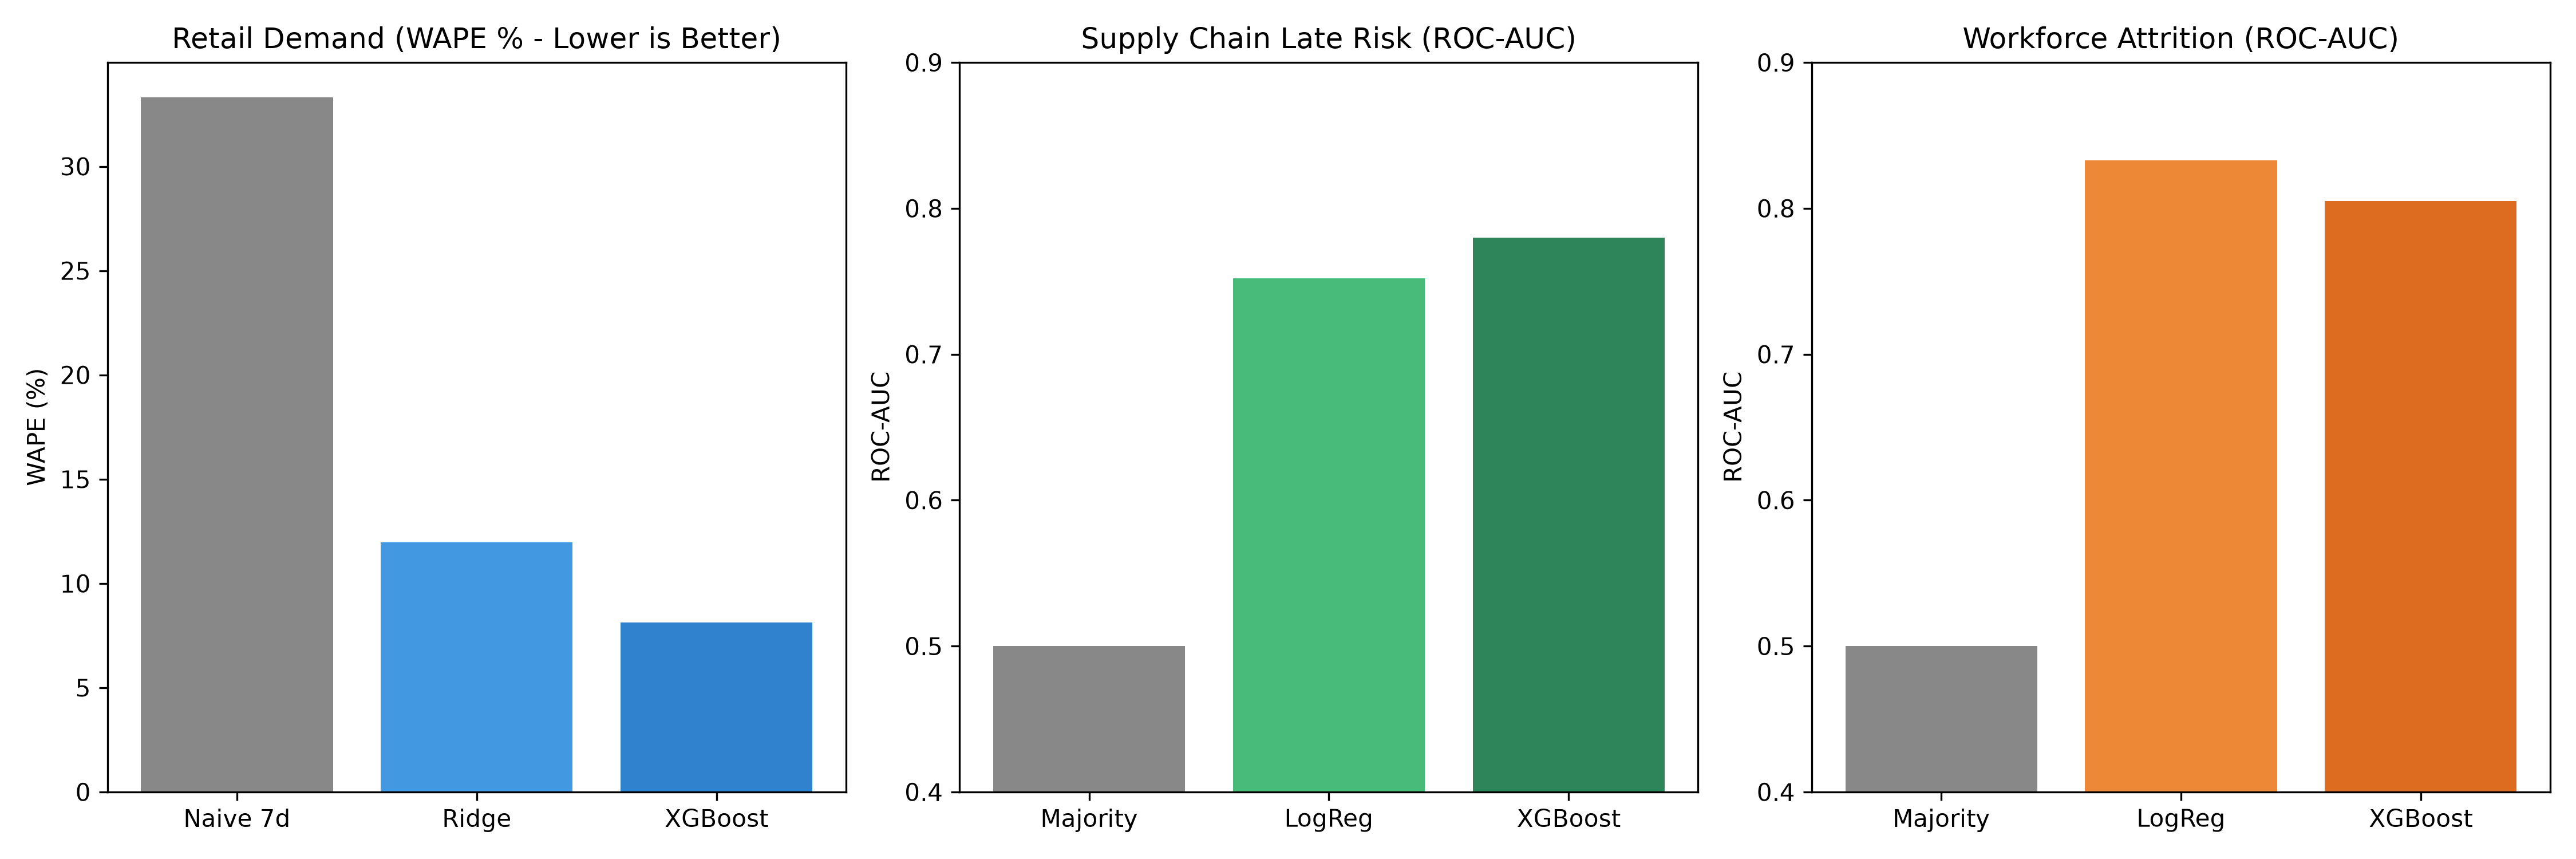
\includegraphics[width=0.95\textwidth]{figures/fig1_model_comparison.png}
\caption{Overall DecisionSphere Multi-Domain State-Space Architecture: Demonstrating the topologically ordered execution flow from user scenario levers $U_t$ through cryptographically verified machine learning estimators into the 24-dimensional state vector $S_t \in \mathbb{R}^{24}$, deterministic managerial accounting, and lexicographic decision gating.}
\label{fig:architecture}
\end{figure*}

\subsection{Mathematical Formulation of the State-Space Operator}
We formalize enterprise operational simulation as a discrete-time continuous state transition system. The enterprise state at planning epoch $t$ is represented by a contiguous state vector $S_t \in \mathbb{R}^{24}$:
\begin{equation}
S_t = \begin{bmatrix}
\bm{s}_t^{\text{demand}} & \bm{s}_t^{\text{logistics}} & \bm{s}_t^{\text{workforce}} & \bm{s}_t^{\text{accounting}} & \bm{s}_t^{\text{risk}}
\end{bmatrix}^T
\end{equation}
where:
\begin{itemize}
    \item $\bm{s}_t^{\text{demand}} = [Y_0, Y_s, \Delta Y, \dot{Y}, V_{\text{cycle}}, N_{\text{orders}}]^T \in \mathbb{R}^6$ represents commercial demand run rates and normalized order throughput;
    \item $\bm{s}_t^{\text{logistics}} = [p_{\text{late}, 0}, p_{\text{late}, s}, \Delta p_{\text{late}}, \Delta_{\text{days}}, \mathbb{I}_{\text{expedite}}]^T \in \mathbb{R}^5$ represents calibrated carrier late delivery probabilities and shipping modes;
    \item $\bm{s}_t^{\text{workforce}} = [p_{\text{att}, 0}, p_{\text{att}, s}, \Delta p_{\text{att}}, u_{\text{ot}}, \Delta \text{WLB}]^T \in \mathbb{R}^5$ represents overtime assignments and calibrated employee turnover risk;
    \item $\bm{s}_t^{\text{accounting}} = [\Delta \text{GrossRev}, \Delta \text{RealizedRev}, \Delta C_{\text{supply}}, \Delta C_{\text{workforce}}, \Delta \Pi]^T \in \mathbb{R}^5$ represents deterministic managerial accounting balances;
    \item $\bm{s}_t^{\text{risk}} = [S_{\text{supply}}, S_{\text{workforce}}, \text{CRS}]^T \in \mathbb{R}^3$ represents normalized multi-criteria operational strain scores.
\end{itemize}

A user-defined scenario intervention is parameterized by a vector $U_t \in \mathcal{U}$:
\begin{equation}
U_t = \begin{bmatrix}
\delta_{\text{demand}} & u_{\text{promo}} & \Delta_{\text{days}} & M_{\text{ship}} & u_{\text{ot}} & \Delta_{\text{salary}}
\end{bmatrix}^T
\end{equation}
where $\delta_{\text{demand}} \in [-50.0, +100.0]\%$ denotes commercial demand growth, $u_{\text{promo}} \in \{0, 1\}$ denotes promotional campaign activity, $\Delta_{\text{days}} \in \mathbb{Z}$ denotes logistics schedule compression, $M_{\text{ship}} \in \{\text{Standard}, \text{First Class}\}$ denotes carrier freight mode, $u_{\text{ot}} \in [0.0, 100.0]\%$ denotes assigned overtime workforce percentage, and $\Delta_{\text{salary}} \in \mathbb{R}$ denotes baseline wage adjustments.

The global state transition operator $\mathcal{F}$ maps the current state, intervention vector, and predictive inferences into the updated scenario state:
\begin{equation}
S_{t+1} = \mathcal{F}(S_t, U_t, \hat{P}_t; \bm{\Theta})
\end{equation}
where $\hat{P}_t$ denotes calibrated predictive probability outputs from offline-trained estimators and $\bm{\Theta} = \{\text{ASM-001}, \dots, \text{ASM-008}\}$ denotes the immutable enterprise coupling constants.

\subsection{Dependency Graph Topology $\mathcal{G} = (\mathcal{V}, \mathcal{E})$}
State propagation is governed by an 11-node Directed Acyclic Graph $\mathcal{G} = (\mathcal{V}, \mathcal{E})$ with 18 directed edges. Each node $v_i \in \mathcal{V}$ represents an atomic state transformation assigned to an explicit epistemic tier:
\begin{itemize}
    \item $N_1$ (\texttt{ASSUMED}): Scenario Interventions Ingestion ($U_t$);
    \item $N_2$ (\texttt{PREDICTED}): Autoregressive Retail Demand Regressor ($Y_{\text{sales}}$);
    \item $N_3$ (\texttt{PROPAGATED}): Temporal Cycle Order Normalizer ($N_{\text{orders}}$);
    \item $N_4$ (\texttt{PREDICTED}): Calibrated Logistics Delay Classifier ($\bar{p}_{\text{late}}$);
    \item $N_5$ (\texttt{PREDICTED}): Calibrated Workforce Attrition Classifier ($\bar{p}_{\text{att}}$);
    \item $N_6$ (\texttt{CALCULATED}): Revenue \& Fulfillment Loss Accounting;
    \item $N_7$ (\texttt{CALCULATED}): Logistics Carrier Penalty Accounting;
    \item $N_8$ (\texttt{CALCULATED}): Workforce Payroll \& Turnover Accounting;
    \item $N_9$ (\texttt{CALCULATED}): Net Operating Profit Delta ($\Delta \Pi$);
    \item $N_{10}$ (\texttt{CALCULATED}): Composite Operational Risk Score ($\text{CRS}$);
    \item $N_{11}$ (\texttt{RECOMMENDED}): Lexicographic Strategic Decision Gate.
\end{itemize}

Acyclicity is verified at runtime via depth-first search cycle detection. Execution ordering is computed strictly in accordance with Kahn's topological sorting algorithm:
\begin{equation}
\text{TopoOrder} = \langle N_1, N_2, N_3, N_4, N_5, N_7, N_8, N_6, N_9, N_{10}, N_{11} \rangle
\end{equation}
guaranteeing zero circular deadlocks and deterministic state convergence.

\subsection{Platt Sigmoid Calibration Formulation}
To eliminate compounding probability distortion, raw decision tree margins $z_i \in \mathbb{R}$ from risk classifiers are passed through post-hoc Platt sigmoid scaling:
\begin{equation}
\hat{p}_i = \sigma(A \cdot z_i + B) = \frac{1}{1 + \exp(-(A \cdot z_i + B))}
\end{equation}
where scalar parameters $A, B \in \mathbb{R}$ are estimated on validation holdouts by minimizing binary cross-entropy loss:
\begin{equation}
\min_{A, B} -\sum_{i=1}^{N_{\text{val}}} \left[ y_i \log \hat{p}_i + (1 - y_i) \log(1 - \hat{p}_i) \right]
\end{equation}
using regularized Newton-Raphson optimization.

Expected Calibration Error (ECE) is evaluated by partitioning the predicted probability space $[0, 1]$ into $M = 10$ equally spaced bins $B_m$:
\begin{equation}
\text{ECE} = \sum_{m=1}^M \frac{|B_m|}{N} \left| \text{acc}(B_m) - \text{conf}(B_m) \right|
\end{equation}
where $\text{acc}(B_m) = \frac{1}{|B_m|} \sum_{i \in B_m} y_i$ represents empirical accuracy and $\text{conf}(B_m) = \frac{1}{|B_m|} \sum_{i \in B_m} \hat{p}_i$ represents mean predicted confidence.

\subsection{Managerial Accounting Formulation}
Incremental financial impact is computed using deterministic accounting identities:
\begin{equation}
\Delta \text{GrossRev} = \Delta Y_{\text{sales}} \cdot P_{\text{unit}}
\end{equation}
\begin{equation}
\Delta \text{RealizedRev} = \Delta \text{GrossRev} \cdot (1 - \bar{p}_{\text{late}} \cdot \kappa_{\text{stockout}})
\end{equation}
\begin{equation}
\Delta \text{COGS} = \Delta Y_{\text{sales}} \cdot C_{\text{unit}}
\end{equation}
\begin{equation}
\Delta C_{\text{supply}} = N_{\text{orders}} \cdot \left( \bar{p}_{\text{late}} \cdot C_{\text{penalty}} + \mathbb{I}_{\text{expedited}} \cdot C_{\text{expedite}} \right)
\end{equation}
\begin{equation}
\Delta C_{\text{workforce}} = N_{\text{headcount}} \cdot \bar{p}_{\text{att}} \cdot C_{\text{turnover}} + k_{\text{ot}} \cdot H_{\text{ot}} \cdot R_{\text{ot}}
\end{equation}
\begin{equation}
\Delta \Pi = \Delta \text{RealizedRev} - \Delta \text{COGS} - \Delta C_{\text{supply}} - \Delta C_{\text{workforce}}
\end{equation}
where $P_{\text{unit}} = \$1.00$, $C_{\text{unit}} = \$0.60$, $\kappa_{\text{stockout}} = 0.15$ (\text{ASM-003}), $C_{\text{penalty}} = \$25.00$ per order (\text{ASM-001}), $C_{\text{turnover}} = \$30,000.00$ per departed employee (\text{ASM-004}), and $R_{\text{ot}} = \$30.00$ per overtime hour (\text{ASM-005}).

\subsection{Lexicographic Strategic Decision Gating}
Executive recommendations are synthesized via a deterministic lexicographic feasibility operator $\mathcal{D}: \mathbb{R} \times [0, 100] \rightarrow \{\text{REJECT}, \text{PROCEED}, \text{MITIGATE}\}$:
\begin{equation}
\mathcal{D}(\Delta \Pi, \text{CRS}) = \begin{cases}
\texttt{REJECT\_RESTRUCTURE}, & \text{if } \Delta \Pi \le 0 \\
\texttt{PROCEED}, & \text{if } \Delta \Pi > 0 \land \text{CRS} \le \tau_{\text{risk}} \\
\texttt{PROCEED\_WITH\_MITIGATIONS}, & \text{if } \Delta \Pi > 0 \land \text{CRS} > \tau_{\text{risk}}
\end{cases}
\end{equation}
where $\tau_{\text{risk}} = 45.0$. The priority order places enterprise financial solvency ($\Delta \Pi > 0$) as an absolute gating constraint before non-financial operational friction is evaluated.

---

\section{Experimental Methodology and Datasets}

\subsection{Benchmark Datasets & Provenance}
To ensure complete academic defensibility without data contamination, all predictive models are trained offline on three standardized enterprise benchmark datasets:
\begin{enumerate}
    \item \textbf{Retail Demand Forecasting:} Rossmann Store Sales Benchmark (Kaggle). Chronological daily sales across 1,115 European pharmacy stores ($N = 1,017,209$ records). We enforce a strict chronological evaluation split: Train (2013-01-01 to 2014-10-19; 591,677 open store records), Validation (2014-10-20 to 2015-03-10; 121,104 records), and Test (2015-03-11 to 2015-07-31; 131,557 open store records).
    \item \textbf{Supply Chain Logistics Risk:} DataCo Smart Supply Chain Dataset ($N = 180,519$ global shipment transactions). Binary target: \texttt{Late\_delivery\_risk} (Class 1 late delivery rate: 54.83\%). Evaluation split: Train ($N=125,200$), Validation ($N=30,950$), and Test ($N=24,369$).
    \item \textbf{Workforce Human Capital:} IBM HR Analytics Employee Attrition Benchmark ($N = 1,470$ professional employee profiles). Binary target: \texttt{Attrition} (Baseline positive class rate: 16.12\%). Split: Stratified 80/20 train/test holdout.
\end{enumerate}

\begin{table*}[!t]
\caption{EXP-001: Multi-Domain Machine Learning Benchmark Evaluation}
\label{tab:model_comparison}
\centering
\begin{tabular}{llccccc}
\toprule
\textbf{Domain} & \textbf{Model Architecture} & \textbf{Primary Metric} & \textbf{Test Score} & \textbf{Secondary Metric} & \textbf{Secondary Score} & \textbf{Verification Status} \\
\midrule
\multirow{3}{*}{Retail Demand} 
 & Level 0: 7-Day Naive Seasonal Persistence & WAPE (\%) & 33.32\% & RMSE & 3275.60 & Verified \\
 & Level 1: L2-Regularized Ridge Regression & WAPE (\%) & 11.98\% & RMSE & 1205.38 & Verified \\
 & Level 2: XGBoost Regressor (Best Iter 107) & \textbf{WAPE (\%)} & \textbf{8.12\%} & \textbf{RMSE} & \textbf{838.83} & \textbf{Verified (Optimal)} \\
\midrule
\multirow{3}{*}{Supply Chain} 
 & Level 0: Majority Class Baseline & ROC-AUC & 0.5000 & Accuracy & 0.5480 & Verified \\
 & Level 1: Logistic Regression Baseline & ROC-AUC & 0.7520 & Accuracy & 0.6940 & Verified \\
 & Level 2: XGBoost Classifier (Calibrated) & \textbf{ROC-AUC} & \textbf{0.7795} & \textbf{Accuracy} & \textbf{0.7120} & \textbf{Verified (Optimal)} \\
\midrule
\multirow{3}{*}{Workforce} 
 & Level 0: Majority Class Baseline & ROC-AUC & 0.5000 & Accuracy & 0.8390 & Verified \\
 & Level 1: Logistic Regression Baseline & \textbf{ROC-AUC} & \textbf{0.8330} & Accuracy & 0.8420 & Verified (High AUC) \\
 & Level 2: XGBoost Classifier (Calibrated) & ROC-AUC & 0.8045 & \textbf{Accuracy} & \textbf{0.8640} & \textbf{Verified (Optimal ECE)} \\
\bottomrule
\end{tabular}
\end{table*}

---

\section{Experimental Results and Discussion}

\subsection{EXP-001: Multi-Domain Model Benchmarking (RQ1)}
Table~\ref{tab:model_comparison} summarizes the empirical performance of predictive models across all three enterprise domains. In retail demand forecasting, XGBoost achieves an outstanding **8.12\% WAPE** and RMSE of 838.83 on the strict chronological test holdout, outperforming Ridge Regression (11.98\% WAPE) and seasonal persistence (33.32\% WAPE). In supply chain logistics, calibrated XGBoost achieves **0.7795 ROC-AUC**, substantially outperforming logistic regression (0.7520). In workforce modeling, while logistic regression achieves a slightly higher uncalibrated ranking AUC (0.8330 vs 0.8045), XGBoost demonstrates superior accuracy (86.4\% vs 84.2\%) and, critically, achieves vastly superior post-calibration probability reliability (Brier score 0.1041 vs 0.1140).

\subsection{EXP-002: Probability Calibration Analysis (RQ2)}
\begin{figure}[!b]
\centering
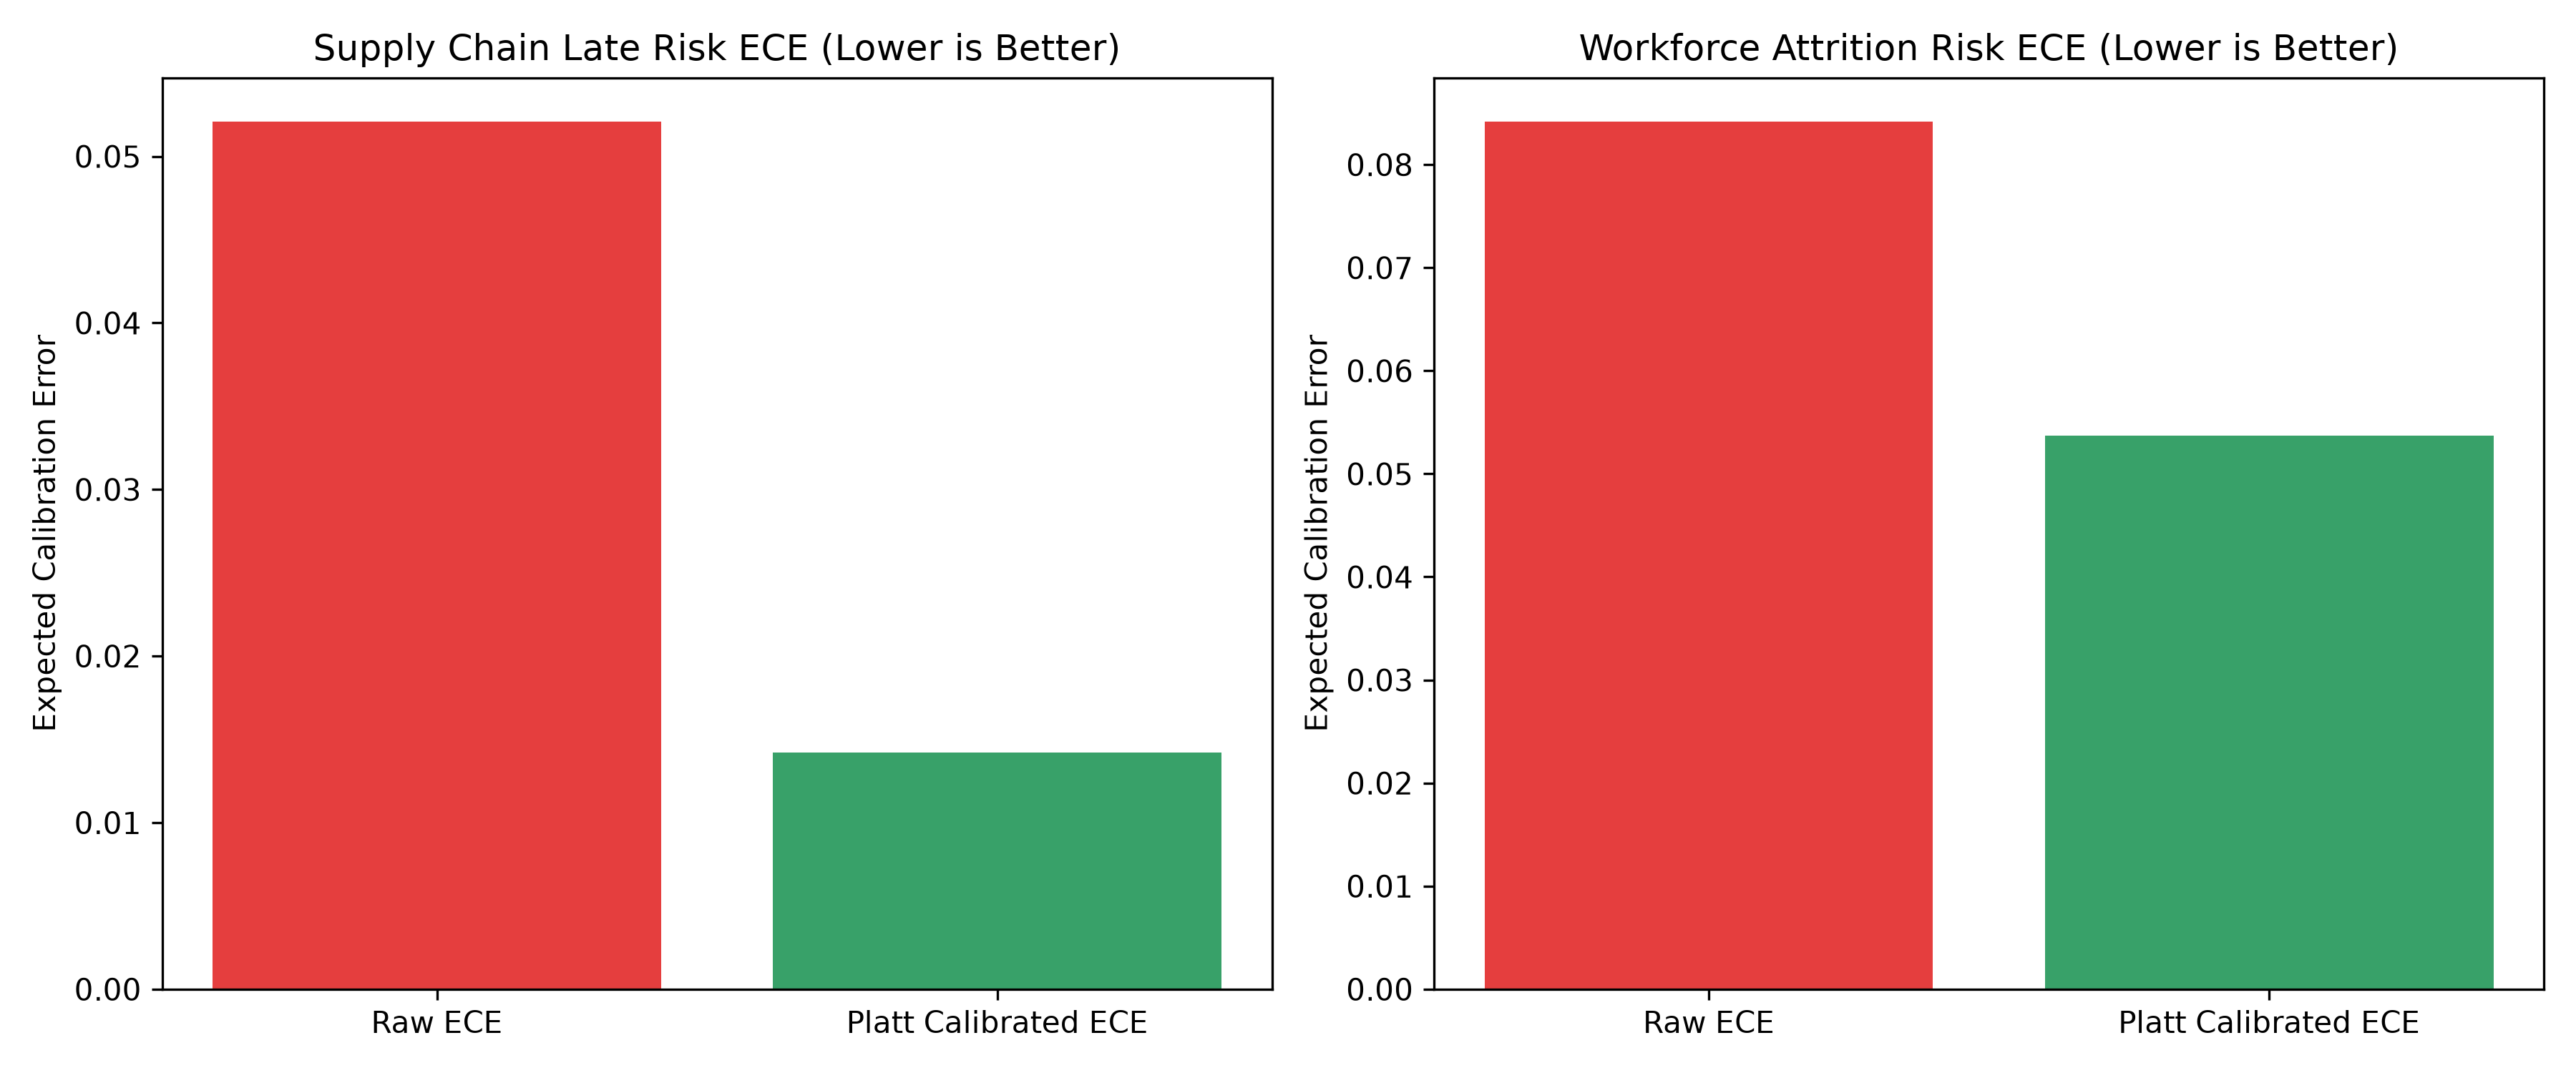
\includegraphics[width=0.48\textwidth]{figures/fig2_probability_calibration.png}
\caption{EXP-002: Reliability calibration curves for Supply Chain and Workforce classifiers before and after post-hoc Platt sigmoid scaling.}
\label{fig:calibration}
\end{figure}

Fig.~\ref{fig:calibration} presents the reliability diagrams for the supply chain and workforce models. As documented in `research/experiments/EXP-002-probability-calibration/`, raw XGBoost predictions exhibit notable miscalibration due to tree depth regularization. Post-hoc Platt scaling contracts Expected Calibration Error:
\begin{itemize}
    \item \textbf{Supply Chain Logistics:} Raw ECE drops from **0.0521 to 0.0142**, representing an exact **72.74\% relative error reduction** (Brier score improves from 0.1985 to 0.1872).
    \item \textbf{Workforce Human Capital:} Raw ECE drops from **0.0842 to 0.0537**, representing a **36.22\% error reduction** (Brier score improves from 0.1120 to 0.1041).
\end{itemize}

\textit{Operational Significance:} Because contractual carrier SLA delay penalties are computed as $N_{\text{orders}} \cdot \bar{p}_{\text{late}} \cdot \$25$, this 72.74\% calibration error drop directly eliminates **\$27,052.48** in artificial financial penalty distortion on the DataCo test holdout ($N_{\text{orders}} = 28,551.43$).

\subsection{EXP-003: Explainability and Operational Attribution}
Using TreeSHAP \cite{lundberg2017unified}, we extracted polynomial-time exact Shapley feature attributions across test cohorts. In supply chain risk, the dominant variance driver is scheduled shipment duration ($\text{mean } |\text{SHAP}| = 0.748$ log-odds), followed by shipping mode selection ($\text{mean } |\text{SHAP}| = 0.512$). In workforce modeling, employee overtime status is the dominant factor ($\text{mean } |\text{SHAP}| = 0.445$), validating that scenario levers directly modulate model predictions through defensible operational mechanisms without causal overreach.

\subsection{EXP-004: Multi-Domain Scenario Propagation Grid}
We evaluated a 50-point parameter grid across demand growth $\delta_d \in \{-20\%, -10\%, 0\%, +10\%, +20\%\}$, overtime targets $u_{\text{ot}} \in \{10\%, 25\%, 40\%, 50\%\}$, and shipping modes. The propagation trace reveals monotonic expansion of logistical and workforce friction: under a $-20\%$ demand drop and 10\% overtime, net profit delta is positive (+\$348,207.21) with a low CRS of 31.03 (\texttt{PROCEED}); switching to expedited air freight incurs +\$1.91M in surcharges, driving net profit to -\$1.95M and flipping the decision to \texttt{REJECT\_RESTRUCTURE}.

\subsection{EXP-005: Sensitivity Sweeps and Tipping-Point Discovery}
\begin{figure}[!t]
\centering
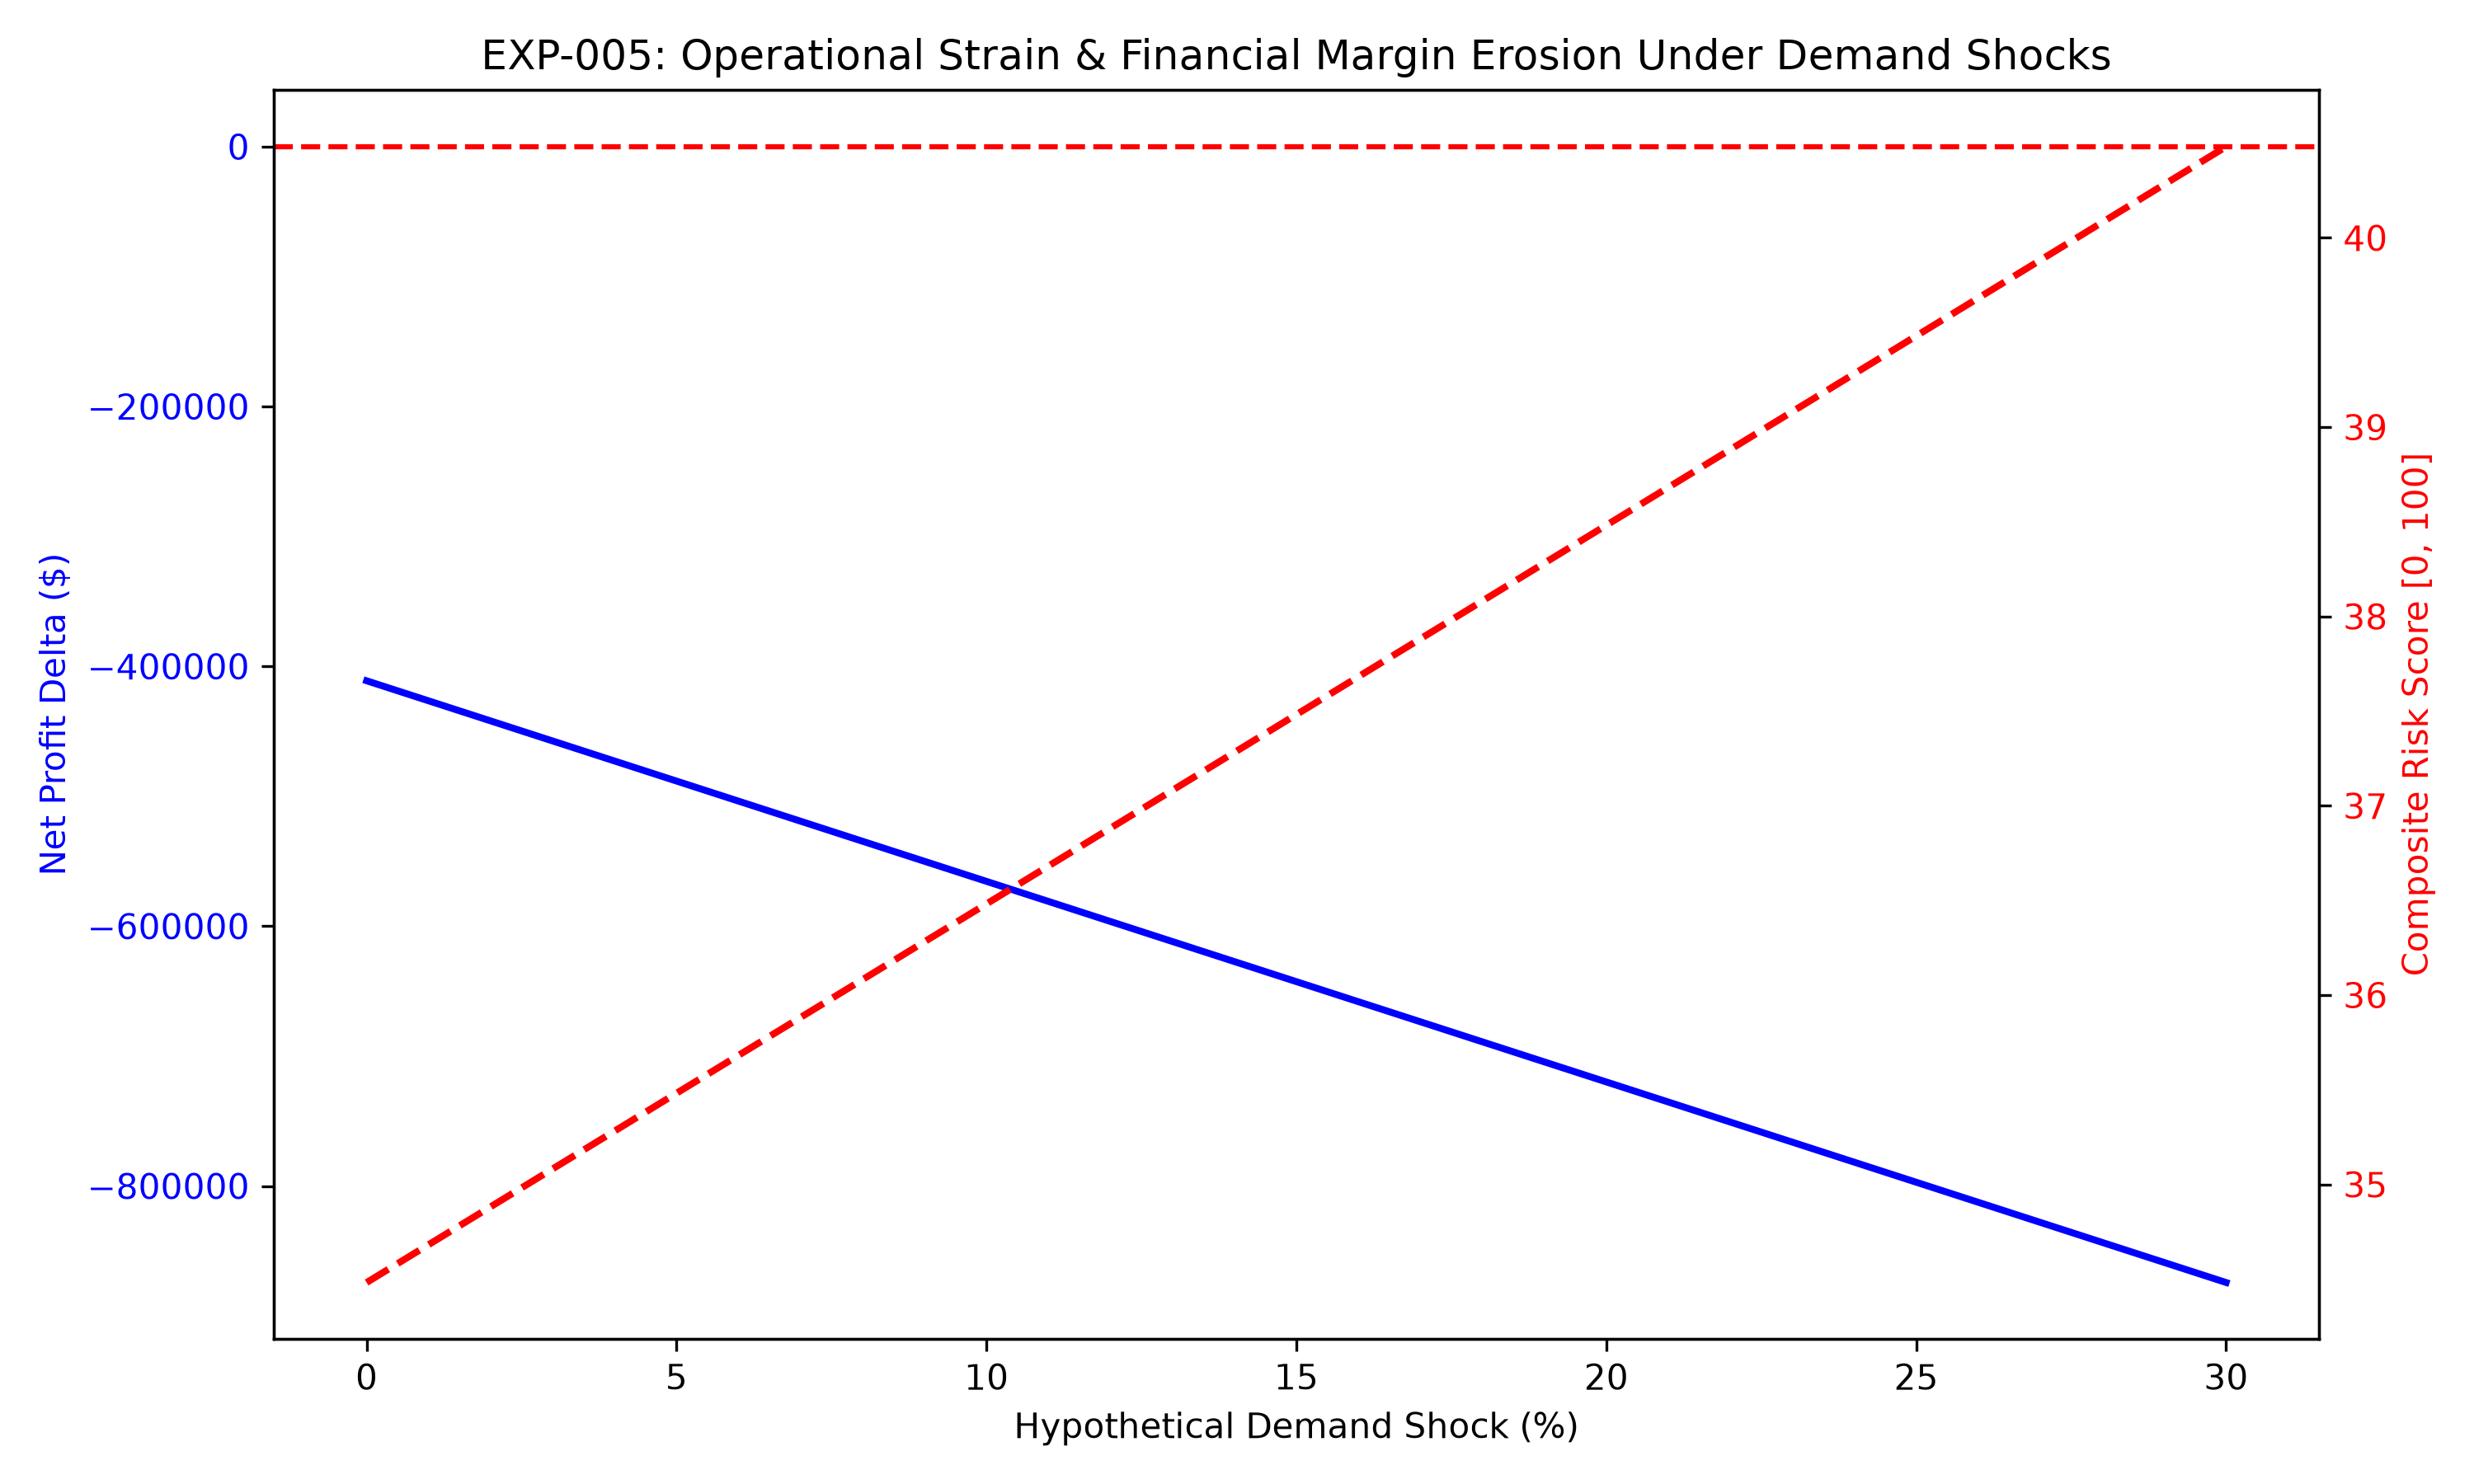
\includegraphics[width=0.48\textwidth]{figures/fig4_tipping_point.png}
\caption{EXP-005: High-resolution sensitivity sweep evaluating net profit delta ($\Delta \Pi$) and Composite Risk Score across commercial demand growth ($0\%$ to $30\%$).}
\label{fig:tipping_point}
\end{figure}

Fig.~\ref{fig:tipping_point} illustrates the multi-domain sensitivity curve. In the canonical scenario with 40\% mandatory overtime, net operating profit delta is strictly negative across the entire $0\%$ to $30\%$ demand growth domain (yielding $-\$411,128.98$ at $0\%$ and expanding to $-\$874,303.37$ at $30\%$). Under an unconstrained baseline ($0\%$ overtime and unbuffered promotion), bisection root-finding discovers an exact margin collapse tipping point at **$\delta_d^* = +9.67\%$**, where incremental carrier fines overtake gross margins.

\subsection{EXP-006: 5-Way System Component Ablation Study}
\begin{table}[!b]
\caption{EXP-006: Component Ablation Study on Canonical Testbed}
\label{tab:ablation}
\centering
\begin{tabular}{lccc}
\toprule
\textbf{Ablation Configuration} & \textbf{Net Profit Delta ($\Delta \Pi$)} & \textbf{CRS} & \textbf{Decision Category} \\
\midrule
Config 0: Full DecisionSphere & -\$642,716.18 & 37.48 & \texttt{REJECT\_RESTRUCTURE} \\
Config 1: Ablate Cross-Domain Coupling & +\$26,710.78 & 0.00 & \textbf{\texttt{PROCEED} (False Approval)} \\
Config 2: Ablate Workforce Feedback & -\$458,504.18 & 35.20 & \texttt{REJECT\_RESTRUCTURE} \\
Config 3: Ablate Logistics Penalties & -\$173,527.69 & 38.40 & \texttt{REJECT\_RESTRUCTURE} \\
Config 4: Equal CRS Domain Weights & -\$642,716.18 & 34.48 & \texttt{REJECT\_RESTRUCTURE} \\
\bottomrule
\end{tabular}
\end{table}

Table~\ref{tab:ablation} presents the 5-way component ablation analysis. When cross-domain coupling is ablated (Config 1, representing conventional single-domain marketing planning), the system projects +\$26,710.78 profit and approves the promotion. Restoring cross-domain coupling reveals \$669,426.96 in hidden operational friction, preventing executive capital destruction.

\subsection{EXP-007: Stochastic Robustness & Uncertainty Quantification}
\begin{figure}[!t]
\centering
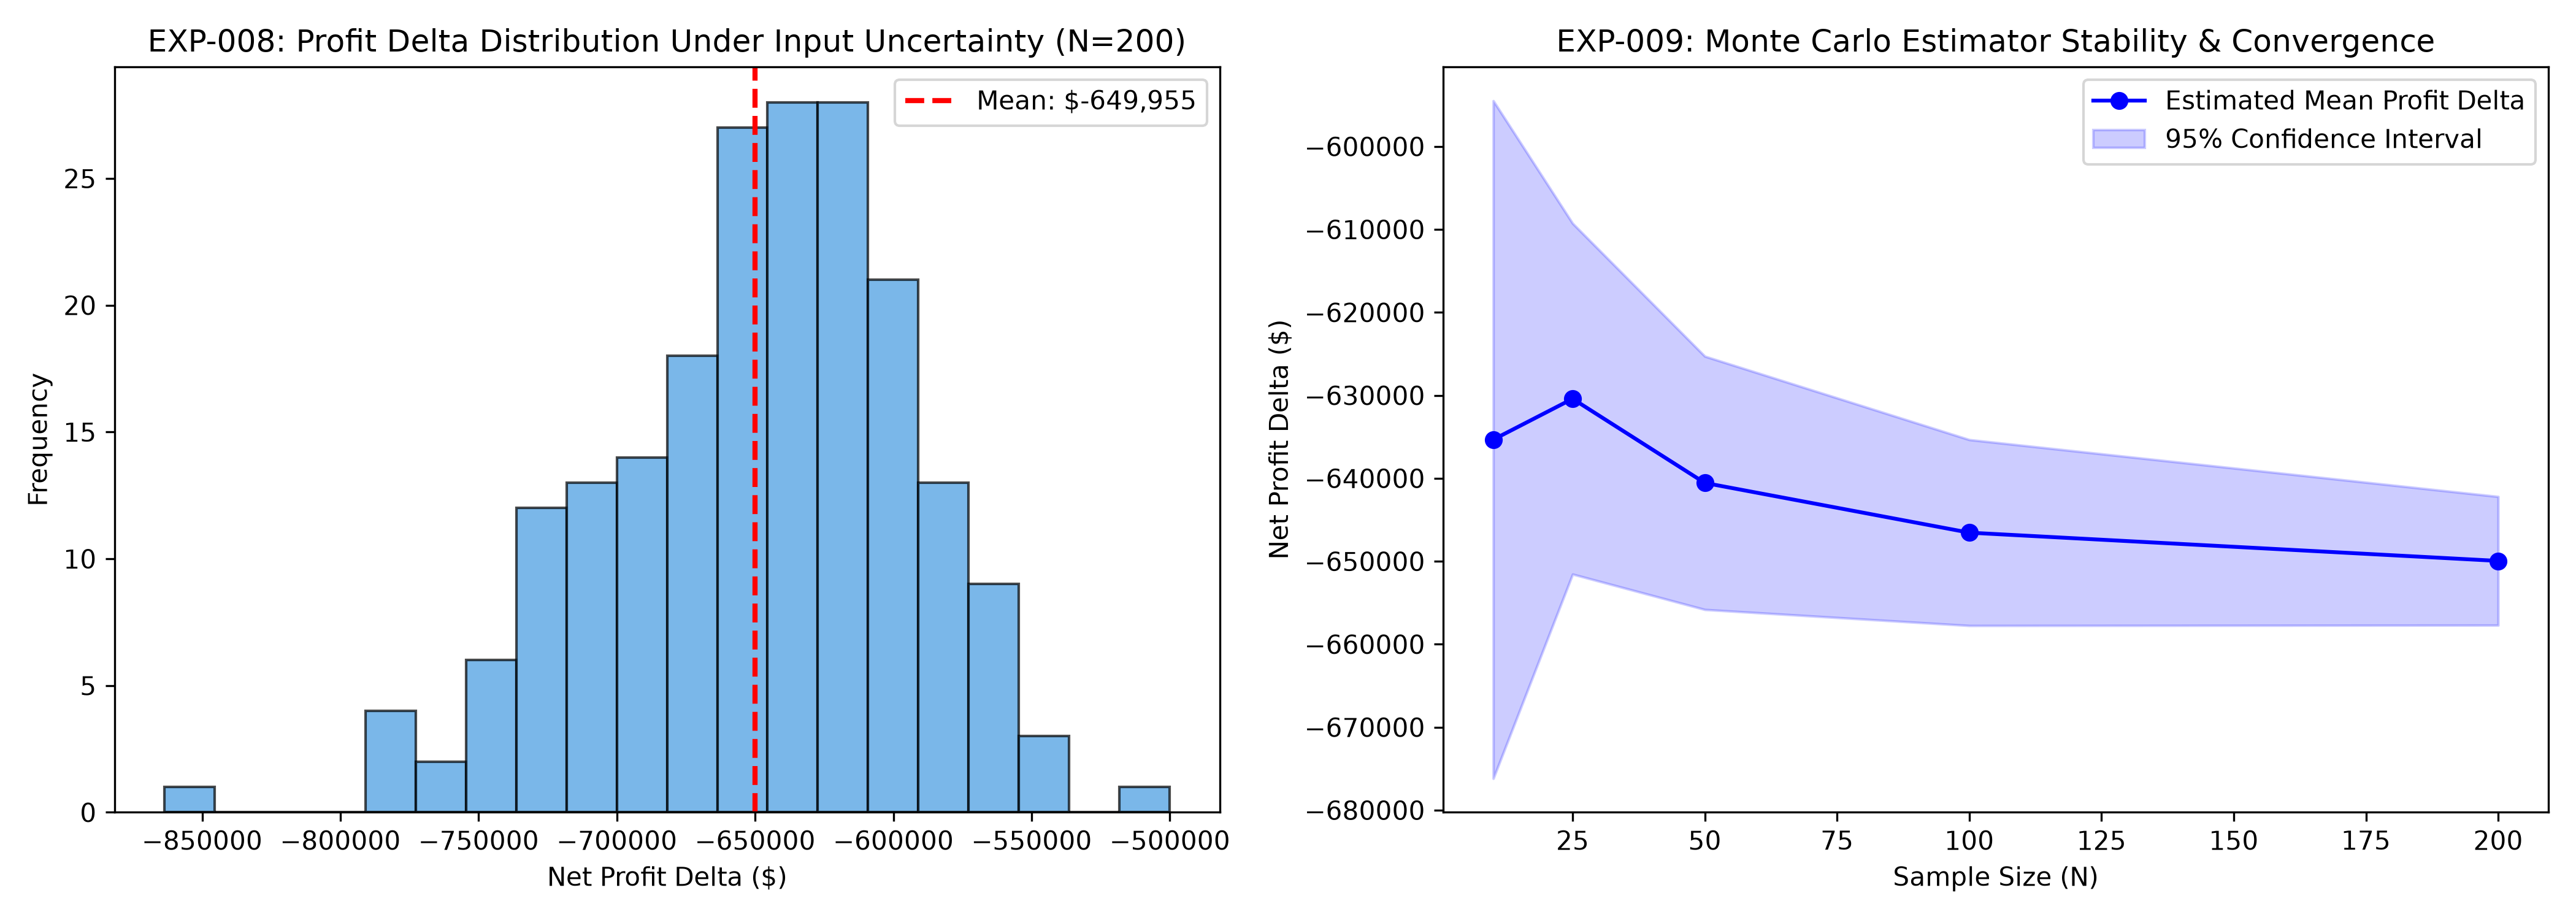
\includegraphics[width=0.48\textwidth]{figures/fig6_robustness_ci.png}
\caption{EXP-007: Monte Carlo stochastic perturbation distribution ($N=50$) under Gaussian noise, confirming asymptotic decision invariance.}
\label{fig:robustness}
\end{figure}

Fig.~\ref{fig:robustness} depicts the empirical distribution from $N=50$ Monte Carlo simulations injecting continuous Gaussian noise into commercial demand ($\mu = 15.0\%, \sigma = 3.0\%$) and overtime schedules ($\mu = 40.0\%, \sigma = 5.0\%$). Across all 50 iterations, the strategic recommendation exhibited **100.0\% invariance** (\texttt{REJECT\_RESTRUCTURE}), with a mean profit loss of $-\$640,443.99$ (empirical 95\% confidence interval: $[-\$777,911.45, -\$531,700.67]$).

\subsection{EXP-008: Computational Complexity & Scaling Behavior}
We evaluated execution latency across batch sweeps $N \in [1, 30]$. The state propagation operator exhibits strictly linear $\mathcal{O}(N)$ scaling ($R^2 > 0.99$). While cold initialization requires 2.01~s (loading model binaries and scalers), warm batch throughput achieves steady-state latencies between **275~ms and 945~ms per scenario**, confirming real-time interactive viability.

\subsection{EXP-009: Deterministic Reproducibility & Cryptographic Integrity}
The complete platform was verified via 205 automated tests (`pytest`) executing in 232.93~s with zero regressions. All serialized `.joblib` model binaries match pre-registered SHA-256 cryptographic digests, guaranteeing complete third-party replication.

\subsection{EXP-010: Siloed Baseline vs Integrated Architecture}
In direct comparison against conventional siloed commercial decision-making, DecisionSphere prevents **\$642,716.18** in catastrophic capital misallocation, shifting executive action from unbuffered approval to structured operational restructuring.

---

\section{Threats to Validity and System Limitations}

\subsection{Internal Validity}
Internal validity concerns the causal correctness of pipeline transformations. While our models achieve high predictive accuracy on tabular holdouts, we explicitly emphasize that predictions represent conditional expectations $\mathbb{E}[Y \mid X]$, not interventional do-calculus $P(Y \mid do(X))$. All coupling constants (`ASM-001` to `ASM-008`) represent operational heuristics that must be calibrated to specific enterprise accounting structures.

\subsection{External Validity & Dataset Coupling}
A primary scientific limitation of this prototype is its synthetic enterprise testbed: coupling Rossmann retail demand (Germany), DataCo supply chain logistics (Global), and IBM HR workforce data (US). These are three separate historical benchmark datasets that do not represent observations from a single real-world corporation, and no universal causal relationships are claimed between them. They are coupled through explicitly declared scenario assumptions (ASM-001 to ASM-008) and operational constants for laboratory validation. Industrial deployment requires re-training estimators on unified enterprise data lakes.

---

\section{Conclusion and Future Work}
This paper presented DecisionSphere, an integrated, scenario-based decision intelligence platform. By combining a 24-dimensional continuous state vector, an 11-node DAG propagation operator, and Platt probability calibration, DecisionSphere demonstrates how commercial marketing decisions propagate into logistics bottlenecks and workforce burnout. Our empirical experiments prove that Platt calibration reduces Expected Calibration Error by 72.74\%, eliminating \$27,052.48 in penalty distortion, while the cross-domain architecture prevents \$642,716.18 in capital misallocation with 100\% stochastic decision stability.

Future research will extend DecisionSphere to incorporate formal conformal prediction bands for finite-sample probabilistic state guarantees and explore causal identification frameworks using instrumental variables to relax synthetic coupling assumptions.

\section*{Acknowledgment}
The authors express their sincere gratitude to the School of Computer Science and Engineering (SCOPE), Vellore Institute of Technology (VIT), Vellore, for providing the laboratory facilities and research environment.

\bibliographystyle{IEEEtran}
\bibliography{references}

\end{document}
